\documentclass[stu,11pt,floatsintext,donotrepeattitle]{apa7}
\usepackage[american]{babel}
\usepackage{newtxtext,newtxmath}
\usepackage{csquotes}
\usepackage[style=apa,backend=biber]{biblatex}
\addbibresource{refs_apa.bib}
\usepackage{graphicx}
\usepackage{booktabs}
\usepackage{threeparttable}
\graphicspath{{figures/}}
\AtBeginDocument{\hypersetup{hidelinks}}

\title{How Groups Build Shared Understanding: Clear Signals Travel, Reading Is Relearned in the Tacit Communication Game}
\shorttitle{How Groups Build Shared Understanding}
\authorsnames{Dylan Wilson}
\authorsaffiliations{Department of Psychological and Brain Sciences, Dartmouth College}
\course{PSYC 63: Experimental Study of Human Interaction}
\professor{Arjen Stolk}
\duedate{November 18, 2026}

\abstract{How does a shared understanding spread through a group? In the Tacit Communication Game, a Sender conveys a hidden goal to a Receiver using only movements on a grid. We ran it as an online tournament in which 16 players met a series of partners over three phases (240 rounds). Players learn two things from feedback: how to produce signals others understand (\emph{learning to signal}) and how to interpret a partner's signals (\emph{learning to read}). If understanding is a shared \emph{code}, both should carry over to a new partner; if it is a \emph{pact} between two people, neither should. On the \emph{asymmetric} account proposed here, clearer signals carry over directly, whereas reading must be relearned with each partner. A neutral reader with no history with the Sender read signals correctly more often in each phase (36\%, 46\%, 61\%), yet real Receivers succeeded less often with a new partner (24\%; McNemar $p = .004$). Signals set a ceiling: when the neutral reader could not read a signal, real partners succeeded only 21\% of the time, against 48\% when it could. Reading also appeared to improve: with signal clarity constant, Receivers meeting a new partner succeeded more often the second time (40\% vs.\ 24\%, $p = .09$). All tournaments shifted toward the form easiest for an outsider to read. Small samples, simulated readers, and partner reunions limit these conclusions. The results suggest that understanding spreads through a group by way of its signals: the forms anyone can read travel and become common.}
\keywords{Tacit Communication Game, conceptual pacts, conventions, mutual understanding, communication, large language models}

\begin{document}
\maketitle

% ======================================================================
\section{Introduction}

Two people who have never met, who cannot speak to each other, and who see the world from different vantage points must somehow come to mean the same thing by the same movement. This is the situation of the Tacit Communication Game \parencite[TCG;][]{deruiter2010}, in which a Sender conveys the location and orientation of a hidden goal to a Receiver using nothing but the movements of a token on a $3 \times 3$ grid. Because no words or conventional signs are available, every successful round is a small act of invention: the Sender must design a movement that will be recognized as communicative rather than instrumental, and the Receiver must infer the intention behind it \parencite{stolk2016}. Pairs typically settle on something like a \enquote{wiggle}, a repeated step from the goal toward a neighboring tile that points the way the goal points \parencite{blokpoel2012}.

That pairs can do this is well established. Much less is known about how such understanding develops in a group: how what two people have worked out between them spreads to others, and how it changes as it spreads. These questions matter beyond the laboratory. Every newcomer to a group, every student entering a discipline, every speaker of a dialect meeting another, faces some version of the problem of whether the understanding built with one person will work with someone else. It matters, too, for how shared signals arise in groups at all. Languages are not invented by committees; they emerge from countless local exchanges between particular people, and yet they end up shared by whole communities. The present study asks how understanding spreads and changes in a group, in a setting where we choose who interacts with whom and where the signals are invented from scratch.

\subsection{Two Kinds of Learning}

A player in the TCG has two different things to learn. As a Sender, the player learns to produce signals: which movements a partner tends to understand. We call this \emph{learning to signal}. As a Receiver, the player learns to interpret signals: what a partner's movements tend to mean. We call this \emph{learning to read}. Both are learned by trial and feedback. After every round the pair finds out whether the Receiver was right, and each player can keep what worked and change what did not, much as learners in signalling games adjust their behavior after each success and failure \parencite{skyrms2010}. Asking how understanding spreads in a group then becomes a concrete question: when a player meets a new partner, which of the two kinds of learning comes along?

\subsection{Code or Pact?}

Two classic positions give opposite answers. On the first, communication works like a \emph{code}: Senders encode a message with a key and Receivers decode it with the same key \parencite[as critiqued by][]{stolk2016}. If shared understanding were a code, then both kinds of learning should carry over: whatever a pair had worked out together should transfer to any new partner who had learned the same key, and switching partners should cost little.

On the second position, understanding is a \emph{conceptual pact}, a temporary agreement between two particular people about how to talk about something \parencite{brennan1996,garrod1987}. Interlocutors coordinate on descriptions that are partner-specific: in referential communication tasks, pairs quickly shorten and stabilize their expressions \parencite{clark1986}, speakers keep using a pact's terms with the partner who shares it more than with a new partner \parencite{brennan1996}, and listeners are slowed when a familiar partner breaks a pact \parencite{metzing2003}. More generally, speakers design utterances for a particular audience \parencite{clark1982}, and on the conceptual alignment account, communicators succeed to the extent that they share a model of what a signal means \emph{to this partner} \parencite{stolk2016}, a shared context that interlocutors actively construct together \parencite{stolk2020}. If understanding were purely a pact, neither kind of learning would carry over, and understanding would reset with each new partner.

Neither position fully fits what is known about groups. Communities whose members rotate partners converge on shared conventions more readily than isolated pairs \parencite{garrod1994,fay2010}, and conventions formed in a community are easier for outsiders to understand than conventions formed in a single pair \parencite{fay2008}. Partner-specific agreements thus seem to give rise, over many interactions, to something more general \parencite{hawkins2023}. How this happens, and which part of a pair's agreement generalizes, has rarely been tested directly. In particular, no study that we know of has separated what Senders learn (how to produce a signal that will be understood) from what Receivers learn (how to interpret the signals they are given) as partners change.

\subsection{The Present Study}

The code and pact accounts treat the two kinds of learning alike: either both carry over or neither does. We propose a third possibility, which we call the \emph{asymmetric} account, on which they come apart. What a Sender learns is how to make a signal clearer, and a clearer signal is clearer to anyone, so learning to signal travels to the new partner. What a Receiver learns is, in large part, how one particular Sender signals, so with a new Sender reading must be relearned, although a Receiver who has done this before may relearn it faster. The two kinds of learning also differ in what they can achieve. A Receiver cannot recover what a signal does not carry, so the clarity of the signal sets a ceiling on understanding that no amount of reading skill can raise. The account differs from a code account in that a new partner must still learn to read, and from a pact account in that the Sender does not start again from nothing. Shared understanding in a group, and with it something like a shared vocabulary of signals, would then be assembled from many pair-level agreements, with the legible parts spreading.

To test these accounts, we rebuilt the TCG \parencite{deruiter2010} as an online tournament in which the experimenter controlled who was paired with whom. Players were paired for ten rounds, re-paired with a new partner for ten rounds, and re-paired again for a final ten rounds. Figure~\ref{fig:hyp} shows what each account predicts for two quantities: how often a neutral reader, who has no history with the Sender, correctly reads the Sender's signals (a measure of what Senders have learned about signalling), and how often the real partner succeeds (which depends on signalling and reading together).

\begin{figure}[t]
\caption{Predictions of Three Accounts of Shared Understanding}
\label{fig:hyp}
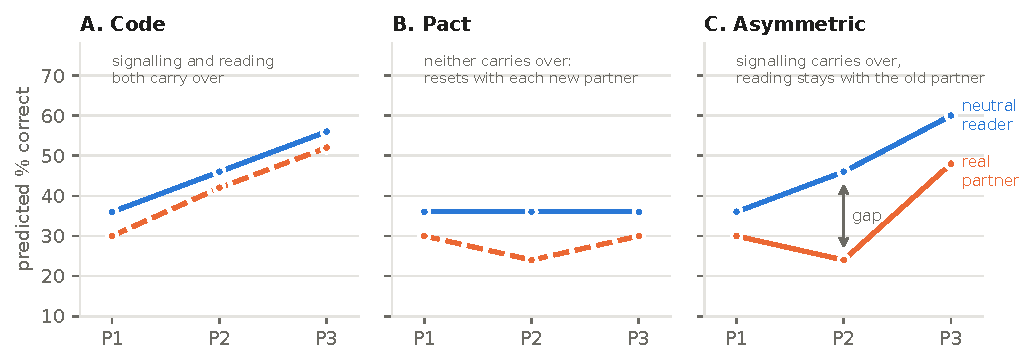
\includegraphics[width=\linewidth]{figH_hypotheses}
\figurenote{Schematic predictions, not data. Blue: proportion of a Sender's signals read correctly by a neutral reader with no history with that Sender (signalling). Orange: success with the real partner (signalling and reading together). P1--P3 are the three partner phases.}
\end{figure}

Our hypothesis, stated in the form of the scientific method, was: \emph{If} players learn with each partner both how to signal and how to read, and learning to signal carries over to a new partner directly while reading must be relearned, \emph{then} we might expect signals to keep getting clearer across partner changes while success drops just after each change. This yields four predictions, each with a null alternative:
\begin{enumerate}
\item[H1a.] Signals become more readable to a neutral reader across phases, even though partners change (H0: legibility does not change across phases).
\item[H1b.] In the phase after a partner switch, real Receivers succeed less often than a neutral reader does on the same signals (H0: real and neutral success do not differ).
\item[H1c.] When early and late signals are crossed with early and late Receivers, later signals improve success more than later Receivers do (H0: Sender and Receiver effects are equal).
\item[H1d.] Each player's signalling style is pulled toward their current partner's style, but not toward the group as a whole (H0: no greater pull from the current partner than from a non-partner).
\item[H1e.] (Exploratory.) At the level of the group, players converge on signal forms that are legible to anyone, rather than on forms specific to their own tournament (H0: the mix of forms does not shift toward legible forms, or shifts toward tournament-specific forms).
\end{enumerate}
A code account predicts H1a but not H1b; a pact account predicts H1b but not H1a. Only the asymmetric account predicts both.

% ======================================================================
\section{Method}

\subsection{Participants}

Sixteen Dartmouth College students took part, all recruited as a convenience sample in and around the college library. They played in three tournaments of six, six, and four players.
% TODO(author): add age range, gender, how consent was obtained, and whether participants were compensated.
Participation was voluntary, players joined under a first name or nickname, and no identifying information was stored with the game logs.

\subsection{Design}

The study used a within-subjects design with \emph{partner phase} (phase 1, first partner; phase 2, new partner; phase 3, new or reunited partner) as the independent variable. The dependent variables were (a) communicative success on each round (the Receiver placed the token on the correct tile with the correct orientation), (b) the legibility of each Sender signal, measured as whether a neutral reader read it correctly, and (c) the position of each Sender signal in a style space (described below). Control variables were held constant across phases: the board, the time limit, the goal set (each goal was used equally often), and the feedback players received.

The partner schedule was not perfectly balanced. In phase 2, every pair was new except one pair in tournament 2. In phase 3, all three pairs in tournament 1 and one pair in tournament 2 were \emph{reunited} with their phase-1 partner, whereas tournament 3 used new partners throughout. We therefore report phase-3 rounds separately for new and reunited partners where it matters.

\subsection{Materials and Apparatus}

We reimplemented the TCG \parencite{deruiter2010}, using the course's \enquote{Crack the Vault} version as a model, as a web application (Node.js server, browser client) so that players could join from their own devices while the experimenter controlled pairing from an administrator dashboard. On each round, one player was the Sender and saw a goal: one of nine tiles and one of eight directions in which the Receiver's triangle should point. The Sender moved a circle with the arrow keys for up to nine seconds (20 seconds on each player's first turn in each role) while the Receiver watched; the Receiver then placed and rotated a triangle. Both players saw only SUCCESS or FAIL. Roles alternated every round. Every key press and its timing were logged.

\begin{figure}[t]
\caption{The Task and the Tournament Design}
\label{fig:game}
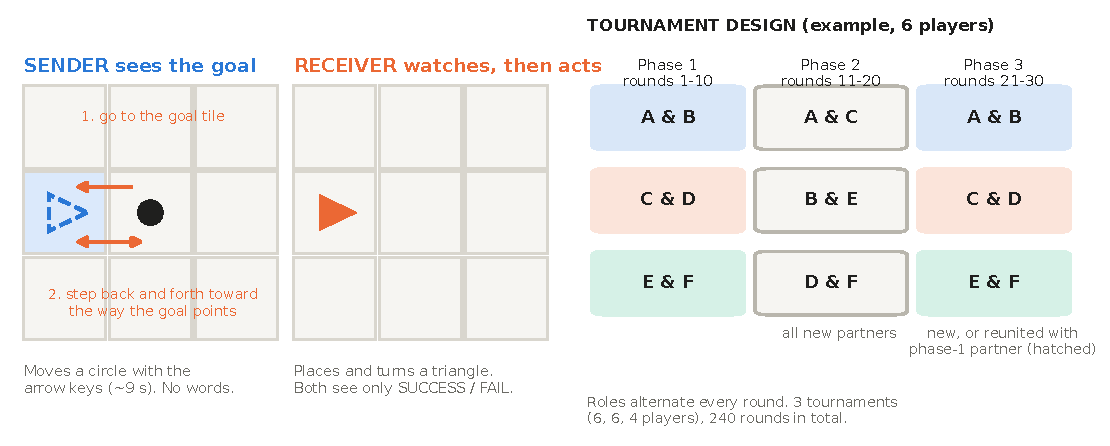
\includegraphics[width=\linewidth]{fig1_game}
\figurenote{Left: one round. The goal (dashed triangle) is the middle-left tile, pointing right; the Sender goes to the goal tile and then steps back and forth toward the way the goal points, and the Receiver places and turns its own triangle. Right: the re-pairing schedule for an example six-player tournament. Hatched pairs in phase 3 are reunions, which occurred in tournament 1 and for one pair in tournament 2.}
\end{figure}

\subsection{Procedure}

Players opened the game on their devices, entered a name, and waited in a lobby. When all players had joined, the experimenter started the tournament. Each tournament had three phases of ten rounds; at each phase boundary, all players saw a message that they were about to play with a different partner, and the server re-paired them according to the schedule (Figure~\ref{fig:game}). The 30 rounds of a tournament took 10 to 11 minutes of play (10.6, 11.3, and 10.0 minutes from the start of the tournament to the last round), or about 21 seconds per round including feedback and the transition to the next round. Of this, active play averaged 15.4 seconds per round ($SD = 5.3$): 8.9 seconds for the Sender's turn and 6.5 seconds for the Receiver's. Across the three tournaments, this produced 240 rounds, 80 in each phase.

\subsection{Analysis}

\subsubsection{Preprocessing}

Each Sender turn's key presses were compressed into readable steps (for example, \enquote{went to top; wiggled top$\leftrightarrow$center $\times 5$; long pause on top; time ran out}). This reduction preserved the final tile in 100\% of turns and the hand-coded strategy in 93\%, but recovered the exact arrow-key sequence in only 59\%, because intermediate tiles and pauses shorter than one second were dropped. No rounds were excluded.

Figure~\ref{fig:tools} summarizes the three measurement tools described next.

\begin{figure}[t]
\caption{The Three Measurement Tools}
\label{fig:tools}
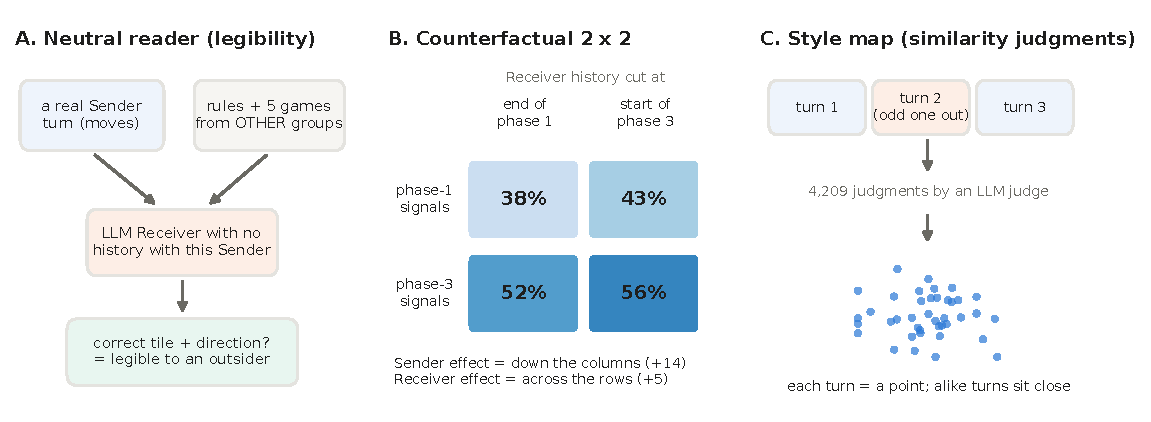
\includegraphics[width=\linewidth]{figT_tools}
\figurenote{(A) A simulated Receiver with no history with the Sender reads each real signal; its accuracy measures legibility. (B) Receivers with early or late histories read early or late signals from players they never partnered; differences down the columns estimate the Sender's contribution and differences across the rows the Receiver's. Cell values are the observed decoding rates. (C) Odd-one-out judgments over triplets of turns are turned into a map in which similar turns lie close together.}
\end{figure}

\subsubsection{Measuring Legibility: A Neutral Reader}

To measure how readable a signal was independent of any particular partner, we used a simulated Receiver: a large language model (GPT-6.1 Terra) given the rules and five complete games from \emph{other} tournaments, and then asked where to place the triangle after reading a Sender turn. Because this reader had no history with any player, its accuracy on a signal reflects how legible the signal is to an outsider. It read all 240 real Sender turns, giving for each turn $t$ a binary legibility score $\ell_t \in \{0, 1\}$ alongside the real outcome $y_t \in \{0, 1\}$.

\subsubsection{Separating Signalling From Reading: A Counterfactual Design}

To separate what Senders and Receivers each contributed, we built a $2 \times 2$ counterfactual. Within each tournament, each real player's history was cut off either at the end of phase 1 (\emph{early Receiver}) or at the start of phase 3 (\emph{late Receiver}). Each version then decoded eight phase-1 signals and eight phase-3 signals sent by \emph{other} players (never signals that player had actually received), for 512 decodes in all. Writing $m_{sr}$ for the decoding rate with signals from phase $s$ and Receiver history $r$ ($E$ = early, $L$ = late), the three quantities of interest are
\begin{align}
\text{Sender effect} &= \tfrac{1}{2}\left[(m_{LE} + m_{LL}) - (m_{EE} + m_{EL})\right], \\
\text{Receiver effect} &= \tfrac{1}{2}\left[(m_{EL} + m_{LL}) - (m_{EE} + m_{LE})\right], \\
\text{Interaction} &= (m_{LL} - m_{LE}) - (m_{EL} - m_{EE}).
\end{align}
The Sender effect asks how much later signals help when the Receiver is held fixed; the Receiver effect asks how much more history helps when the signals are held fixed; and the interaction asks whether late signals work especially well for late Receivers, as a shared convention would predict. Confidence intervals were obtained by resampling Receivers (3,000 bootstrap samples).

\subsubsection{Measuring Style: An Embedding Built From Similarity Judgments}

Rather than rely on hand-coded strategy labels, we built a map of signalling style from similarity judgments, following the odd-one-out approach used to map human object concepts \parencite{hebart2020}. A language-model judge saw three Sender turns, each with its own goal, and named the one whose signalling strategy was the odd one out. We collected 2,649 such triplets over all 240 turns plus 1,560 two-choice probes (4,209 judgments) and fitted a three-dimensional embedding by maximum likelihood, so that turns judged alike sit close together. Each turn $i$ receives a position $\mathbf{x}_i \in \mathbb{R}^3$. When the judge names $k$ as the odd one out of $\{i, j, k\}$, it is in effect saying that $i$ and $j$ are the most similar pair, and the model assigns this choice the probability
\begin{equation}
P(k \text{ odd} \mid \mathbf{x}) = \frac{\exp(-\lVert \mathbf{x}_i - \mathbf{x}_j \rVert^2)}{\exp(-\lVert \mathbf{x}_i - \mathbf{x}_j \rVert^2) + \exp(-\lVert \mathbf{x}_i - \mathbf{x}_k \rVert^2) + \exp(-\lVert \mathbf{x}_j - \mathbf{x}_k \rVert^2)}.
\end{equation}
The positions maximize the summed log probability of all judgments; three dimensions predicted held-out judgments best. For analyses of change, we removed the goal from each turn's position,
\begin{equation}
\mathbf{r}_t = \mathbf{x}_t - \frac{1}{|G_t|}\sum_{u \in G_t} \mathbf{x}_u,
\end{equation}
where $G_t$ is the set of turns with the same goal as turn $t$ (each goal occurred eight times), so that distance reflects style rather than goal.

The embedding's internal validity was acceptable. The judge gave the same answer on 84\% of reshuffled triplets (a ceiling); the embedding predicted 70\% of held-out triplets (chance 33\%) and 81\% of held-out pairwise probes (chance 50\%); and a new turn placed from ten judgments predicted 72\% of its other judgments. Its three axes were readable: signalling a direction versus simply going to the goal, stepping toward versus away from the goal direction, and marking the center versus wiggling at the goal. Because the judge's prompt originally listed example strategies, we repeated the procedure with the examples removed.

\subsubsection{Inferential Tests}

Changes in success and legibility across phases were tested with logistic regression on phase, $\operatorname{logit} P(y_t = 1) = \beta_0 + \beta_1\,\text{phase}_t$, and with $\chi^2$ tests. Differences between a neutral reader and the real Receiver on the same signals were tested with McNemar's test, and group differences in proportions with Fisher's exact test. The pull of a partner's style was tested by regressing each player's next turn on their own previous turn and their current partner's latest turn,
\begin{equation}
\mathbf{r}_{p,\,t+1} = a_1\,\mathbf{r}_{p,\,t} + a_2\,\mathbf{r}_{q(p),\,t} + \boldsymbol{\varepsilon},
\end{equation}
where $q(p)$ is $p$'s current partner, pooling the three dimensions, with standard errors clustered by player ($n = 224$ turns with a preceding turn). A third term, the mean of $p$'s own past successful turns ($a_3$), was added in an extended model. A placebo model replaced the partner with a random non-partner from the same tournament. Because each Sender contributed several turns, we checked the main legibility and success effects with generalized estimating equations (logistic, exchangeable correlation, clustered by Sender). For the gap between reader and partner, each turn contributed two outcomes, one for the neutral reader ($N = 1$) and one for the real partner ($N = 0$):
\begin{equation}
\operatorname{logit} P(\text{correct}) = \beta_0 + \beta_1 N + \sum_{k=2}^{3}\left(\gamma_k\,[\text{phase} = k] + \delta_k\,N\,[\text{phase} = k]\right),
\end{equation}
so that $\delta_2$ tests whether the gap after the first switch is larger than in phase 1. To test for group-specific signal forms, we used a rule-based label of each Sender turn's form (computed from its moves) (for example, a wiggle toward the goal direction, a sideways wiggle, or simply going to the goal) and compared the probability that two turns in the same tournament and phase share a form with the same probability when tournament labels were shuffled within phase (1,000 permutations).

\subsubsection{A Generative Model}

To test whether the partner pull could account for the group-level pattern, we fitted a generative model in which each player's next turn is a weighted combination of their own last turn, their partner's last turn, and their own past successful turns, and success depends on how legible the signal is and how well it matches what the Receiver has come to expect. We then simulated the model 300 times on each tournament's real partner schedule. As a separate comparison, we asked whether large language models given a player's history could predict that player's next move, and let them play whole tournaments in closed loop.

% ======================================================================
\section{Results}

\subsection{Success Fell, Then Rose}

Across all players, real success was 29\% in phase 1 (23 of 80 rounds), 24\% in phase 2 (19 of 80), and 49\% in phase 3 (39 of 80), $\chi^2(2) = 12.52$, $p = .002$. Success increased over phases, odds ratio (OR) $= 1.58$ per phase, $p = .008$. The fall from phase 1 to phase 2 was not itself statistically reliable (Fisher's exact $p = .59$), whereas the rise from phase 2 to phase 3 was ($p = .002$).

\subsection{Signals Became Clearer, but New Partners Misread Them (H1a, H1b)}

The neutral reader decoded Senders' signals correctly 36\%, 46\%, and 61\% of the time in phases 1--3 (29, 37, and 49 of 80), a steady increase, OR $= 1.67$ per phase, $p = .002$ (Figure~\ref{fig:gap}). This supports H1a: signals became more legible even though partners changed.

\begin{figure}[t]
\caption{Legibility Rose Steadily While Real Success Dipped After the First Switch}
\label{fig:gap}
\centering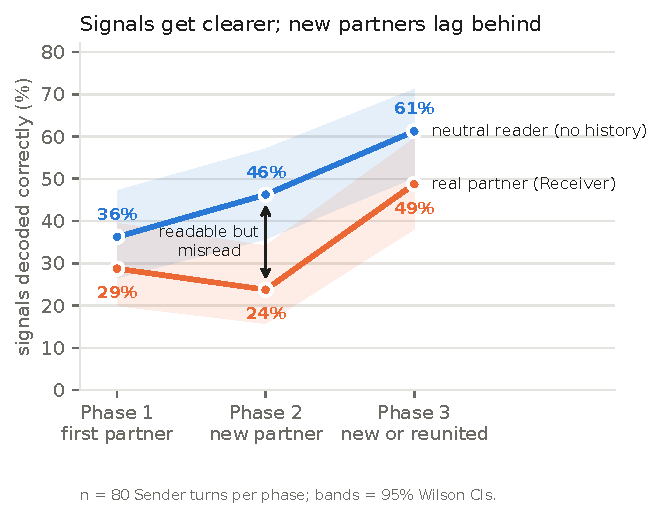
\includegraphics[width=0.78\linewidth]{figG_gap}
\figurenote{The same signals, read by a neutral reader with no history (blue) and by the players' real partners (orange). Bands are 95\% Wilson confidence intervals; $n = 80$ Sender turns per phase.}
\end{figure}

In phase 2, the gap between the two was large. On the same 80 signals, the neutral reader succeeded on 37 and the new partner on 19; in 27 rounds the neutral reader was right and the partner wrong, and in only 9 the reverse, McNemar $p = .004$. In phase 1 there was no reliable gap (29 versus 23; discordant 17 versus 11, $p = .34$), and in phase 3 it was smaller (49 versus 39; 16 versus 6, $p = .052$). These effects held when repeated turns by the same Sender were taken into account: legibility still rose across phases (OR $= 1.67$, $p = .004$), success still rose (OR $= 1.58$, $p = .015$), and the phase-2 gap remained (OR $= 2.76$, $p = .005$). Crucially, the gap was larger in phase 2 than in phase 1 ($\delta_2$: OR $= 1.96$, $p = .044$), whereas the phase-3 gap did not differ from phase 1 ($p = .67$), so the neutral reader was not simply better than people across the board. The gap appeared in tournaments 1 and 2 (43\% vs.\ 23\% and 60\% vs.\ 23\%) and was small in tournament 3 (30\% vs.\ 25\%). This supports H1b: after a switch, Senders were producing clearer signals than before, but their new partners read them differently. The gap did not open at once. In the first five rounds with a new partner, real Receivers and the neutral reader did about equally well (31\% vs.\ 34\% of 35 rounds); in the last five, the neutral reader rose to 57\% while real Receivers fell to 17\%.

\subsection{Later Signals Helped; the Receiver Effect Was Uncertain (H1c)}

In the counterfactual design (Figure~\ref{fig:cf}), the same Receivers decoded later signals better than earlier ones by 14 percentage points, 95\% CI [5, 22]. Giving a Receiver more history helped less and not reliably, 5 points [$-4$, 14]. Late signals did not work especially well for late Receivers, interaction $-1$ point [$-12$, 11]. Cell means were 38\% (early signals, early Receivers), 43\% (early signals, late Receivers), 52\% (late signals, early Receivers), and 56\% (late signals, late Receivers). The Sender effect was reliable and the Receiver effect was not, but the two did not differ reliably from each other: the difference was 9 points, 95\% CI [$-7$, 24]. H1c is therefore supported in direction only. Because these Receivers were simulated by a language model given a player's history, this test also cannot show whether the players themselves became better readers.

\begin{figure}[t]
\caption{Counterfactual Decoding Separates Signalling From Reading}
\label{fig:cf}
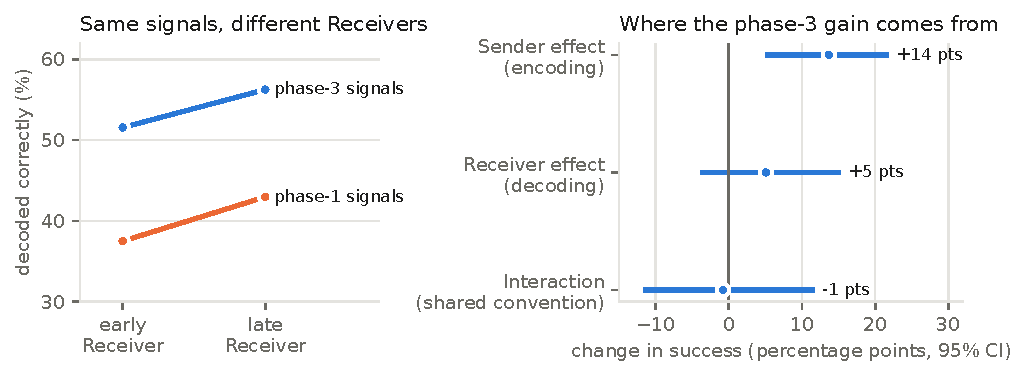
\includegraphics[width=\linewidth]{fig3_counterfactual}
\figurenote{Left: success for each combination of signal phase and Receiver history. Right: main effects and interaction with 95\% confidence intervals (Receivers resampled).}
\end{figure}

\subsection{Signals Set a Ceiling, and Reading Improved Within It (Exploratory)}

The following analyses were not planned and should be read as exploratory. We first asked how far real success depended on the signal itself, by splitting rounds according to whether the neutral reader had read the signal correctly (Table~\ref{tab:ceiling}). When it had not, real partners succeeded 21\% of the time (26 of 125), and this figure barely moved across phases (22\%, 21\%, 19\%), even though by phase 3 many pairs had played together before. When it had, real partners succeeded 48\% of the time (55 of 115), Fisher's exact $p < .001$. Partners found the correct tile equally often in both cases (83\%); what unreadable signals failed to convey was the direction (25\% correct vs.\ 53\%). A signal that an outsider cannot read is thus seldom rescued by familiarity with the Sender: the signal sets a ceiling on what any reader can recover.

\begin{table}[t]
\caption{Real Partners' Success by Whether a Neutral Reader Could Read the Signal}
\label{tab:ceiling}
\begin{tabular}{lccc}
\toprule
Signal & Phase 1 & Phase 2 & Phase 3 \\
\midrule
Readable to the neutral reader & 41\% (12/29) & 27\% (10/37) & 67\% (33/49) \\
Unreadable to the neutral reader & 22\% (11/51) & 21\% (9/43) & 19\% (6/31) \\
\bottomrule
\end{tabular}
\end{table}

Within that ceiling, reading appeared to improve. For readable signals, real success went from 41\% to 27\% to 67\% across phases. The fairest comparison is between Receivers meeting a new partner in phase 2 and in phase 3, because the neutral reader found those two sets of signals about equally clear (46\% of 70 vs.\ 48\% of 40). Real Receivers nevertheless did better the second time, 40\% versus 24\% (16 of 40 vs.\ 17 of 70), Fisher's exact $p = .09$; on signals the neutral reader could read, they succeeded on 53\% (10 of 19) versus 25\% (8 of 32). This is what one would expect if people become better at reading someone new, though the difference is not reliable and the phase-3 new pairs came only from tournaments 2 and 3. Receivers also differed from one another more than Senders did: individual success rates ranged from 7\% to 67\% as a Receiver and from 20\% to 53\% as a Sender.

\subsection{Reunions: An Important Confound}

In phase 3, reunited pairs succeeded more often than new pairs, 57\% versus 40\% (23 versus 16 of 40), though this difference was not reliable (Fisher's exact $p = .18$; Figure~\ref{fig:reunion}). The reunited Senders' signals were, however, also more legible to the neutral reader, 75\% versus 48\% ($p = .021$). Reunions were concentrated in tournament 1, so the reunion advantage may reflect better Senders in that tournament rather than a pact that was resumed. New partners in phase 3 still did better than partners in phase 1 (40\% versus 29\%), so the phase-3 rise is not only a reunion effect.

\begin{figure}[t]
\caption{Phase-3 Success and Legibility for New and Reunited Partners}
\label{fig:reunion}
\centering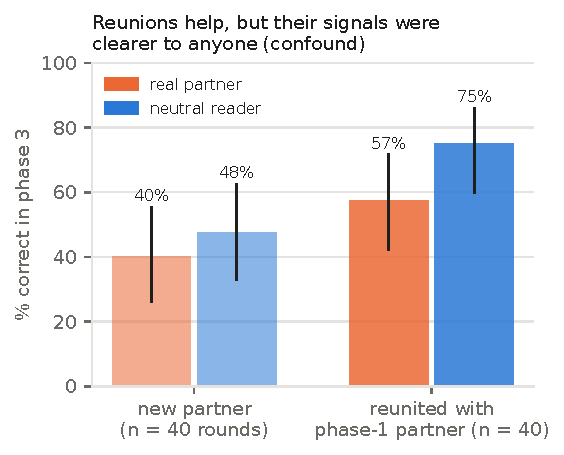
\includegraphics[width=0.6\linewidth]{figR_reunion}
\figurenote{Error bars are 95\% Wilson confidence intervals; $n = 40$ rounds per group.}
\end{figure}

\subsection{What Signals Looked Like}

The style embedding supported one robust distinction: turns that try to signal a direction versus \enquote{still} turns that simply go to the goal; two clusters described the data better than one, and more clusters did not improve the fit. A four-way description, written by reading raw turns, remained informative (Figure~\ref{fig:emb}): \emph{pointers} step back and forth between the goal and the neighbor in the goal direction (42\% success); \emph{right axis, unclear end} turns move along the correct line but leave which end is the head ambiguous (36\%); \emph{still or minimal} turns pause and mark the goal (42\%); and \emph{busy or circling} turns loop through several neighbors and usually time out (16\%).

\begin{figure}[t]
\caption{A Map of Signalling Style Built From Similarity Judgments}
\label{fig:emb}
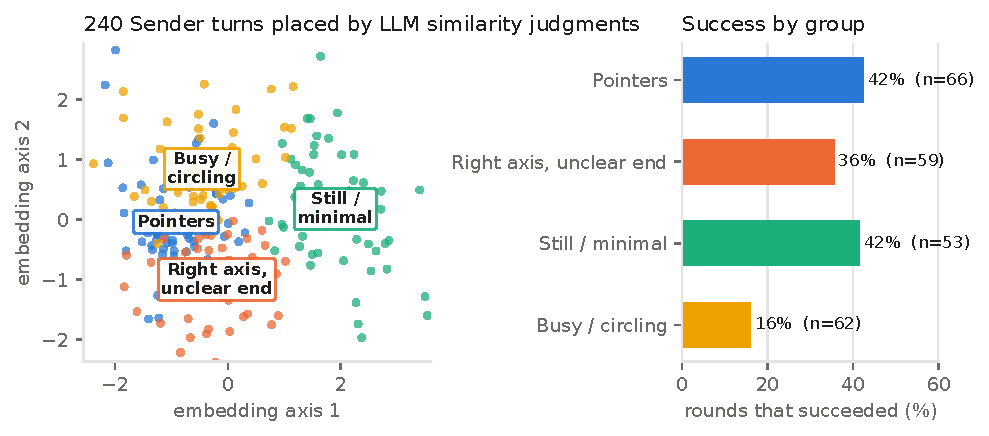
\includegraphics[width=\linewidth]{fig4_embedding}
\figurenote{Left: all 240 Sender turns in the embedding, colored by a four-way k-means split and labeled with verbal descriptions. Right: success for each group.}
\end{figure}

\subsection{Did Groups Develop Shared Signals? (H1e)}

If each tournament were building its own small language, turns within a tournament should come to share forms more often than turns from different tournaments. They did not. The probability that two turns in the same tournament and phase used the same form was no higher than when tournament labels were shuffled (0.20 vs.\ 0.20, permutation $p = .31$). Instead, the tournaments moved in the same direction (Figure~\ref{fig:lex}). The share of turns that signalled a direction at all rose from 69\% in phase 1 to 88\% in phase 2, and the \emph{pointer} form, a wiggle from the goal toward the way the goal points, rose from 15\% to 36\% of turns (Fisher's exact $p = .003$), led by tournaments 1 and 2. This was the most legible form in the game: the neutral reader decoded pointer turns correctly 71\% of the time against 39\% for all other forms ($p < .001$), and real partners succeeded with them 57\% of the time. The shift did not settle into a fixed convention; in phase 3 the pointer share fell back to 21\% as some players returned to simply marking the goal. Because tournaments never met, this convergence cannot reflect copying between groups; it is better described as many pairs independently arriving at the form that is easiest for anyone to read. H1e was thus supported for the direction of change, though not for a stable group convention.

\begin{figure}[t]
\caption{Signal Forms by Tournament and Phase}
\label{fig:lex}
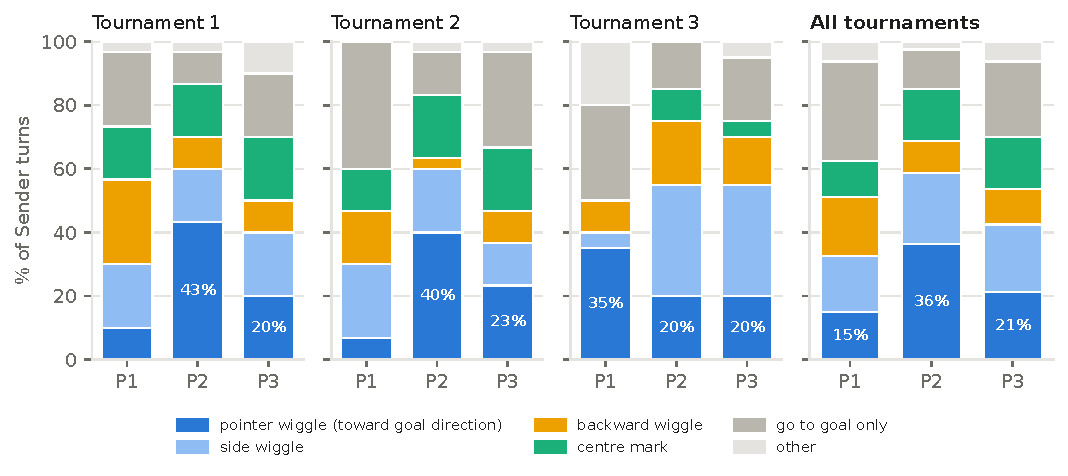
\includegraphics[width=\linewidth]{figL_lexicon}
\figurenote{Rule-based form label of every Sender turn. The pointer wiggle (dark blue) was the most legible form for the neutral reader (71\% correct vs.\ 39\% for other forms).}
\end{figure}

\subsection{Each Player Was Pulled Toward Their Current Partner (H1d)}

In the style space, partners' turns were always closer to each other than to non-partners' (mean distance in phases 1--3: partners 2.21, 1.66, 1.73; non-partners in the same tournament 2.52, 1.77, 2.12). Regressing each player's next turn on their own previous turn and their current partner's latest turn gave weights of 0.25 ($p < .001$) and 0.13 ($p = .002$). Substituting a random non-partner gave $-0.08$ ($p = .004$; Figure~\ref{fig:model}). The partner pull was present in phase 1 (0.16, $p = .014$) and phase 3 (0.17, $p = .041$) and absent in phase 2 (0.01), and it replicated with the judge that saw no example strategies (0.14, $p = .009$). Adding the player's own past successful turns gave weights of 0.21 (own), 0.12 (partner), and 0.17 (own successes). The models were modest in size: own and partner turns together explained 9.4\% of the variance in a player's next turn, and the full model 10.6\% (9.3\% when predicting held-out tournaments).

\begin{figure}[t]
\caption{The Style-Update Model}
\label{fig:model}
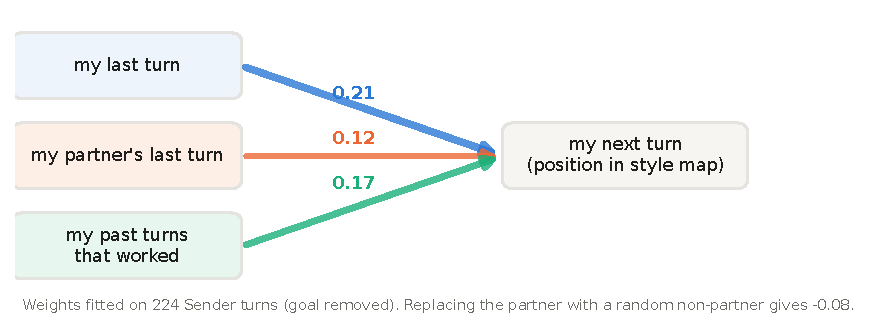
\includegraphics[width=\linewidth]{figM_model}
\figurenote{Fitted weights on a player's next turn in the style map (goal removed; 224 turns). Arrow width is proportional to weight.}
\end{figure}

We found no sign of a group-wide style. All distances shrank in phase 2, including between players in different tournaments who never met, which points to a shared shift at that stage rather than social copying (Figure~\ref{fig:conv}). A judge could not tell which tournament a turn came from (50\%, chance 50\%). Nor did styles lock in: the size of a player's change from one turn to the next did not shrink with games played together once phase was controlled (slope $+0.001$ per game, $p = .96$), and was only slightly smaller after a success (1.60 versus 1.76). H1d was therefore supported in its pairwise form: styles were pulled toward the current partner, not toward the group.

\begin{figure}[t]
\caption{Convergence in Signalling Style}
\label{fig:conv}
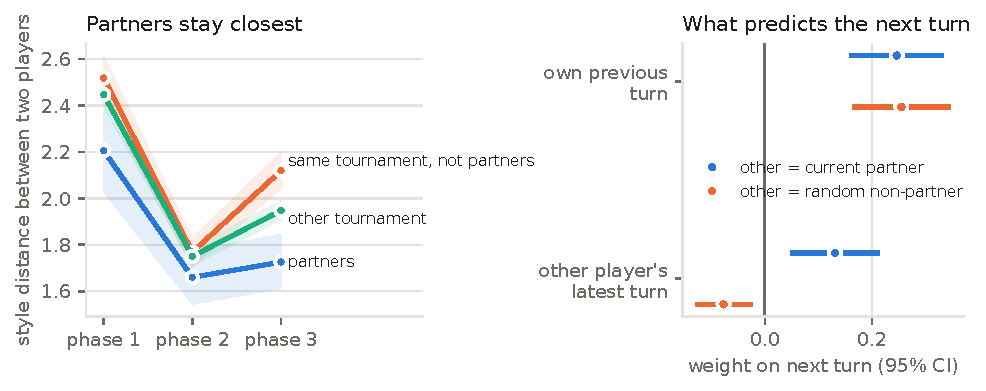
\includegraphics[width=\linewidth]{fig5_convergence}
\figurenote{Left: style distance between two players' turns in the same phase. Right: weights on a player's next turn, with 95\% confidence intervals clustered by player.}
\end{figure}

\subsection{Simulating the Model}

The fitted model reproduced the partner alignment but not the success curve (Figure~\ref{fig:sim}). Simulated on the real schedules, partners ended up closer in style than non-partners, and removing the partner pull erased this gap. Simulated success, however, was 31\%, 38\%, and 34\% in phases 1--3 against the real 29\%, 24\%, and 49\%. The reason appears to lie in the style map rather than the model: legibility estimated through the three embedding dimensions was flat (about 47\% in every phase), whereas the neutral reader showed 36\%, 46\%, and 61\%. The three-number style map does not capture what makes a signal readable.

\begin{figure}[t]
\caption{The Fitted Model Simulated on the Real Partner Schedules}
\label{fig:sim}
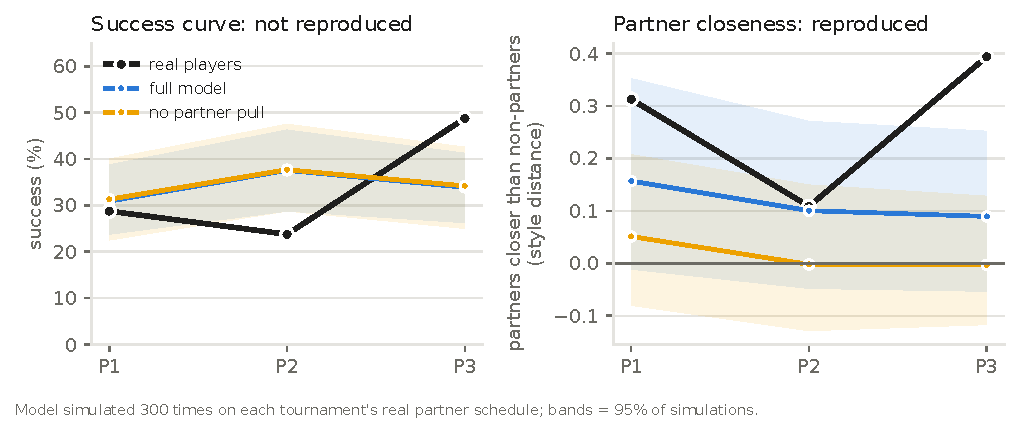
\includegraphics[width=\linewidth]{figS_sim}
\figurenote{Real players (black) against 300 simulations of the full model (blue) and of the model without partner pull (yellow). Bands contain 95\% of simulations.}
\end{figure}

\subsection{Language Models as Models of Players}

Given each player's real history and games from the other tournaments, GPT-6.1 Terra predicted the Sender's strategy 57\% of the time and the Receiver's interpretation 63\% of the time, above a history-free baseline (43\% and 49\%; Figure~\ref{fig:llm}). Claude Sonnet 5.5 (50\%, 57\%) and Claude Haiku 5.5 (41\%, 43\%) did worse. A judge preferred Terra's predicted turn over the player's previous turn as a match to the actual turn 70\% of the time, against 53\% for a same-goal turn by another player. With the goal held fixed, however, Terra's prediction was judged closer to the player's current turn than the player's real next turn was (58\%, $p = .013$): the model predicts less change than people make. When language models played entire tournaments, simulated pairs succeeded 48\%, 68\%, and 60\% of the time in phases 1--3, with no cost of switching partners. Simulated players coordinated far more easily than people did.

\begin{figure}[t]
\caption{Language Models as Models of Players}
\label{fig:llm}
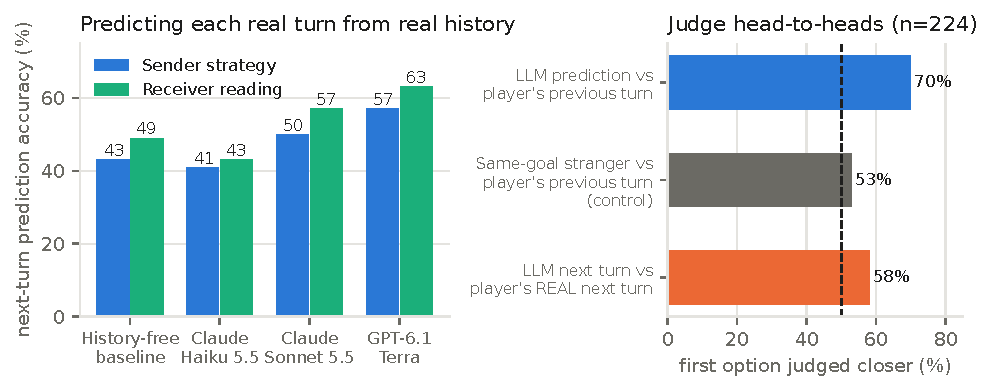
\includegraphics[width=\linewidth]{fig6_llm}
\figurenote{Left: accuracy of next-move predictions from real history (leave-one-tournament-out). Right: judge comparisons on 224 Sender turns.}
\end{figure}

% ======================================================================
\section{Discussion}

We asked how shared understanding spreads through a group: whether it behaves like a code, in which everything a pair has learned would transfer to any partner, or like a pact, in which it would reset with each one. The data fit neither account alone. Signals became steadily more legible to a reader who had never met the Sender, as a code account predicts, yet real partners misread these clearer signals in the phase after a switch, as a pact account predicts. In the counterfactual decomposition, later signals reliably improved reading and Receiver experience did not, although the two effects could not be told apart statistically. We therefore reject the null hypotheses for H1a and H1b, for the pairwise form of H1d, and, for the direction of change, H1e; H1c was supported in direction only. The evidence favors a version of the asymmetric account in which clearer signals carry over to new partners directly, while reading has to be relearned with each partner. It does not show that reading fails to improve. The exploratory analyses suggest instead that signals set a ceiling on understanding, and that within this ceiling Receivers became better at reading new partners.

\subsection{How Shared Signals Develop in a Group}

These results suggest one way that conceptual pacts \parencite{brennan1996,garrod1987} could give rise to community conventions \parencite{garrod1994,fay2010}. Each pair negotiates its own agreement, but the agreement has two sides. The Sender's side, in becoming more explicit, becomes readable to outsiders; the Receiver's side is fitted to one Sender and must be rebuilt with the next, perhaps more quickly each time. As players rotate, the forms that anyone can read are the ones that survive contact with a new partner. This mirrors the finding that signs refined in a community are easier for outsiders to interpret than those refined in an isolated pair \parencite{fay2008}, and it is consistent with the conceptual alignment framework \parencite{stolk2016}: the dip after a switch is exactly what one expects if Receivers interpret signals through a model of what this particular partner means. On this view, joint context is constructed within pairs \parencite{stolk2020}, while its most legible products are what a group comes to share. The group-level data fit this picture. No tournament developed a dialect of its own; rather, pairs in every tournament moved toward the same pointer form, the one an outsider could read most easily. This resembles what is thought to happen in emerging languages, where forms that are transparent to newcomers are favored as they pass between many speakers \parencite{fay2008}. A shared vocabulary, on this account, need not be agreed upon by anyone. It can emerge because legible forms survive each change of partner and idiosyncratic ones do not.

The account also makes a prediction about newcomers, a special case of the same process. Someone joining a group should be understood before they understand others: their own signals, if clear, will be read, but they will need time to learn each partner's way of signalling. The pull toward the current partner's style, present in phases 1 and 3, shows one mechanism by which a pair's styles become matched, though in our short sessions this did not add up to a group-wide convention.

\subsection{Limitations}

Several limitations constrain these conclusions. On internal validity, the phase-3 reunions confound partner familiarity with tournament: reunions occurred mostly in tournament 1, whose Senders were also more legible, so we cannot cleanly separate a resumed pact from better signallers. The \enquote{neutral} reader was not a blank slate: to learn the game it saw five complete games from other tournaments, including their later phases. It is therefore an outsider familiar with how other groups played, and because the tournaments converged on similar forms, part of the rise in legibility may reflect growing resemblance to those groups' later signals; a language model may also simply favor transparent forms such as the pointer. The counterfactual Receivers were simulated by a language model, and language models proved too stable to reproduce human variability, adapting less than people do; the Receiver contribution may therefore be underestimated. The counterfactual test did not show that Senders contributed more than Receivers: the Receiver effect was positive, its interval included an effect as large as the Sender effect, and the Receivers in that test were simulated. We therefore cannot say how much people's reading improved, only that the exploratory comparisons point toward improvement. The style map was built from a language model's judgments; repeating the procedure without example strategies reduces, but does not remove, the concern that the map reflects the judge's assumptions. And the three-dimensional map loses information that direct judgments retain. Finally, we ran several tests without correcting for multiple comparisons, the key gap-by-phase interaction was only just significant ($p = .044$), and the group-level analysis (H1e) was exploratory; these results should be treated as a first test rather than a settled finding.

On external validity, the sample was small (16 players, 240 rounds) and drawn by convenience from a university library, and several effects were not statistically clear, including the dip itself. The task is a wordless, nine-second laboratory game; real communication involves words, shared histories, and rich context, and the extent to which our findings generalize to conversation is unknown.

\subsection{Future Directions}

Three steps follow. First, more tournaments with a balanced schedule, in which no pair is reunited and every player meets several new partners, would remove the main confound and test whether a group convention eventually emerges. Second, testing real people as the counterfactual Receivers, reading signals from players they have never met, would replace the simulated decoder with a human one. Third, measuring legibility directly from decoder results, rather than through the three-dimensional style map, should let the generative model reproduce the success curve and not only partner alignment.

\subsection{Conclusion}

When strangers build a shared language without words, what they learn has two halves that behave differently. Senders learn to make their meaning legible, and that legibility travels to new partners. Receivers learn to read a particular partner, and that reading must be learned again with the next, though perhaps more easily each time. What a signal does not carry, no reader can recover. Across a group, pairs converge on the forms anyone can read. Shared signals in a group, like the words of an emerging language, may thus be assembled from many pair-level agreements, with the most legible forms being the ones that spread.

\printbibliography

\appendix
\section{Supplemental Materials: Analysis Code}

The code for the online game, all analysis scripts, and the source of this report are publicly available at \url{https://github.com/dylan518/tcg-ladder}. To protect participants' privacy, the game logs are not included in the repository; they are available from the author on request. The main scripts are:
\begin{itemize}
\item \texttt{engine.js}, \texttt{tournament.js}, \texttt{public/}: the online game, tournament pairing, and logging.
\item \texttt{analysis/tokenize\_games.py}, \texttt{analysis/models/readable.py}: preprocessing of key presses into readable steps.
\item \texttt{analysis/models/cf\_encode\_decode.py}: neutral-reader legibility and the $2 \times 2$ counterfactual decoding.
\item \texttt{analysis/models/strategy\_embed.py}, \texttt{analysis/models/eval\_embeddings.py}: triplet judgments and the style embedding.
\item \texttt{analysis/models/reading\_ceiling.py}: exploratory analyses of the signal ceiling and of reading with new partners.
\item \texttt{analysis/models/convergence.py}: distance analyses and the style-update regressions.
\item \texttt{analysis/label\_strategies.py}: hand-coded signal forms (group-level form analysis).
\item \texttt{analysis/models/group\_model.py}: the generative model and its simulations.
\item \texttt{analysis/models/fullgame\_sonnet.py}, \texttt{analysis/models/llm\_validity.py}: language models as models of players.
\item \texttt{paper/make\_figures.py}, \texttt{paper/make\_figures\_v2.py}: all figures.
\end{itemize}

\end{document}
